\documentclass[10pt]{beamer}

\usepackage{natbib}

\usetheme[progressbar=frametitle]{metropolis}
\usepackage{appendixnumberbeamer}

\usepackage{booktabs}
\usepackage[scale=2]{ccicons}

\usepackage{pgfplots}
\usepgfplotslibrary{dateplot}

\usepackage{xspace}
\newcommand{\themename}{\textbf{\textsc{metropolis}}\xspace}

\usepackage{amsmath, bm}
\usepackage[ruled,vlined]{algorithm2e}
\usepackage[utf8]{inputenc}
\usepackage{amssymb}

\newcommand*{\QEDA}{\hfill\ensuremath{\blacksquare}}%
\newcommand*{\QEDB}{\hfill\ensuremath{\square}}%



\title{Generative Adversarial Networks}
\subtitle{}
% \date{\today}
\date{}
\author{Davi Barreira}
\institute{FGV - Escola de Matemática Aplicada}
% \titlegraphic{\hfill\includegraphics[height=1.5cm]{logo.pdf}}
\usepackage{caption}
\captionsetup[figure]{font=footnotesize}

\begin{document}

\maketitle

\begin{frame}{Table of contents}
  \setbeamertemplate{section in toc}[sections numbered]
  \tableofcontents[hideallsubsections]
\end{frame}

\AtBeginSection{}
\section[Introdução]{Introdução}
\begin{frame}[fragile]{Introdução}

	\textbf{Generative Adversarial Networks} (GAN)
	foram originalmente introduzidas por \citet{goodfellow2014}.
	Essas redes são utilizadas com o objetivo de gerar
	dados sintéticos realísticos a partir de dados reais.

    \begin{figure}[H]
        \centering
        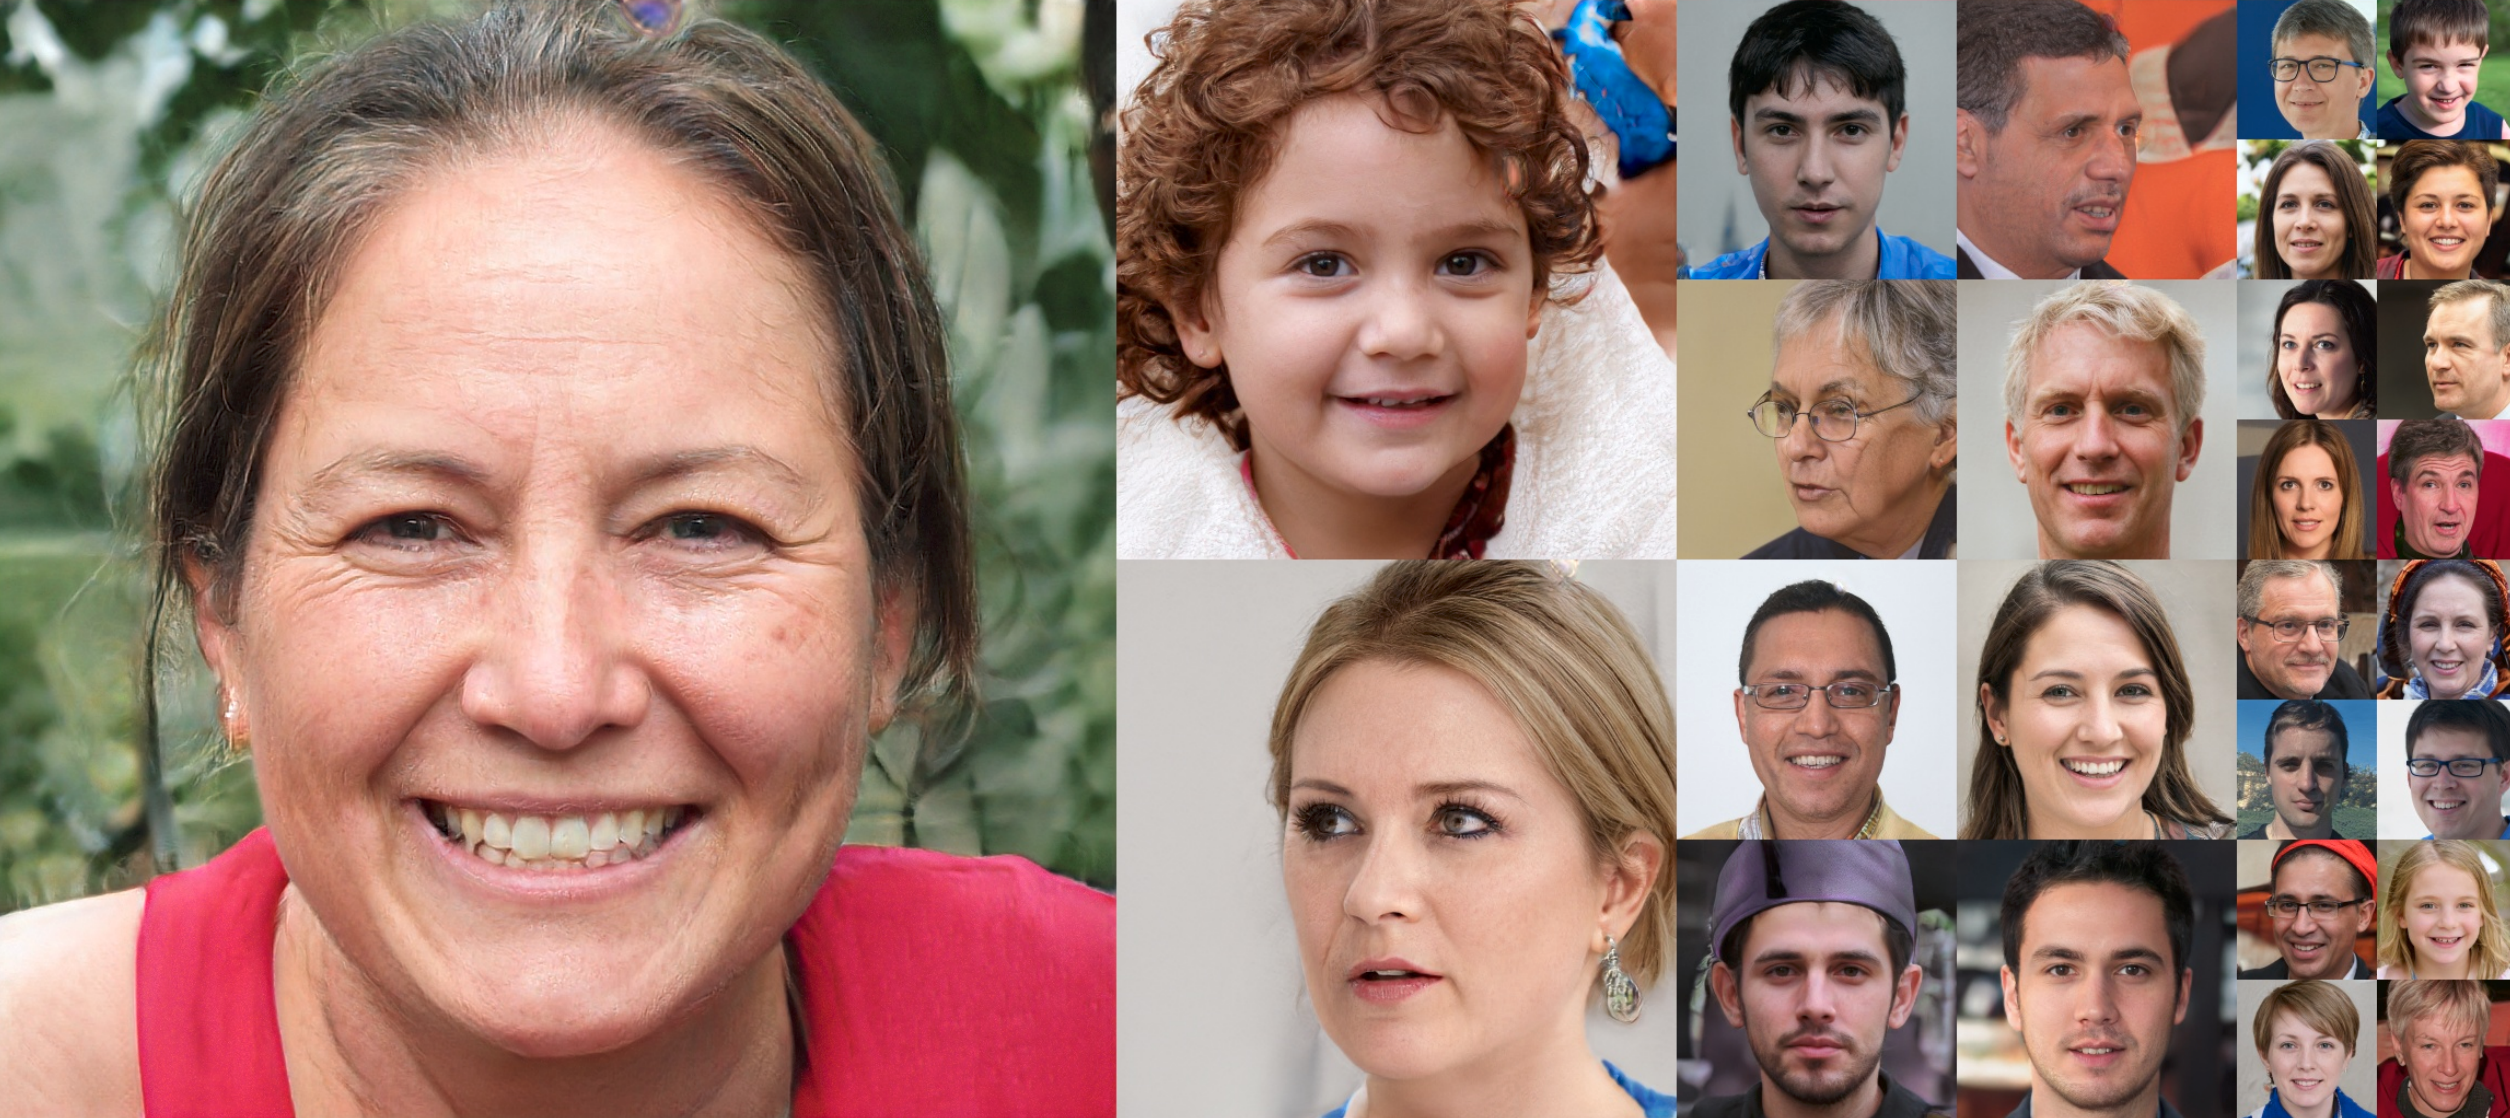
\includegraphics[width=8cm]{images/gans-faces.png}
        \caption{Faces geradas por GANs
        \footnote{Faces geradas por \citet{karras2018}}.}
    \end{figure}

\end{frame}

\begin{frame}[fragile]{Introdução}

	A geração de novas amostras sintéticas tem diferentes utilidades,
	como aprendizado semi-supervisionado, geração de exemplos
	adversariais, \textit{style transfer}, entre outros.

    \begin{figure}[H]
        \centering
        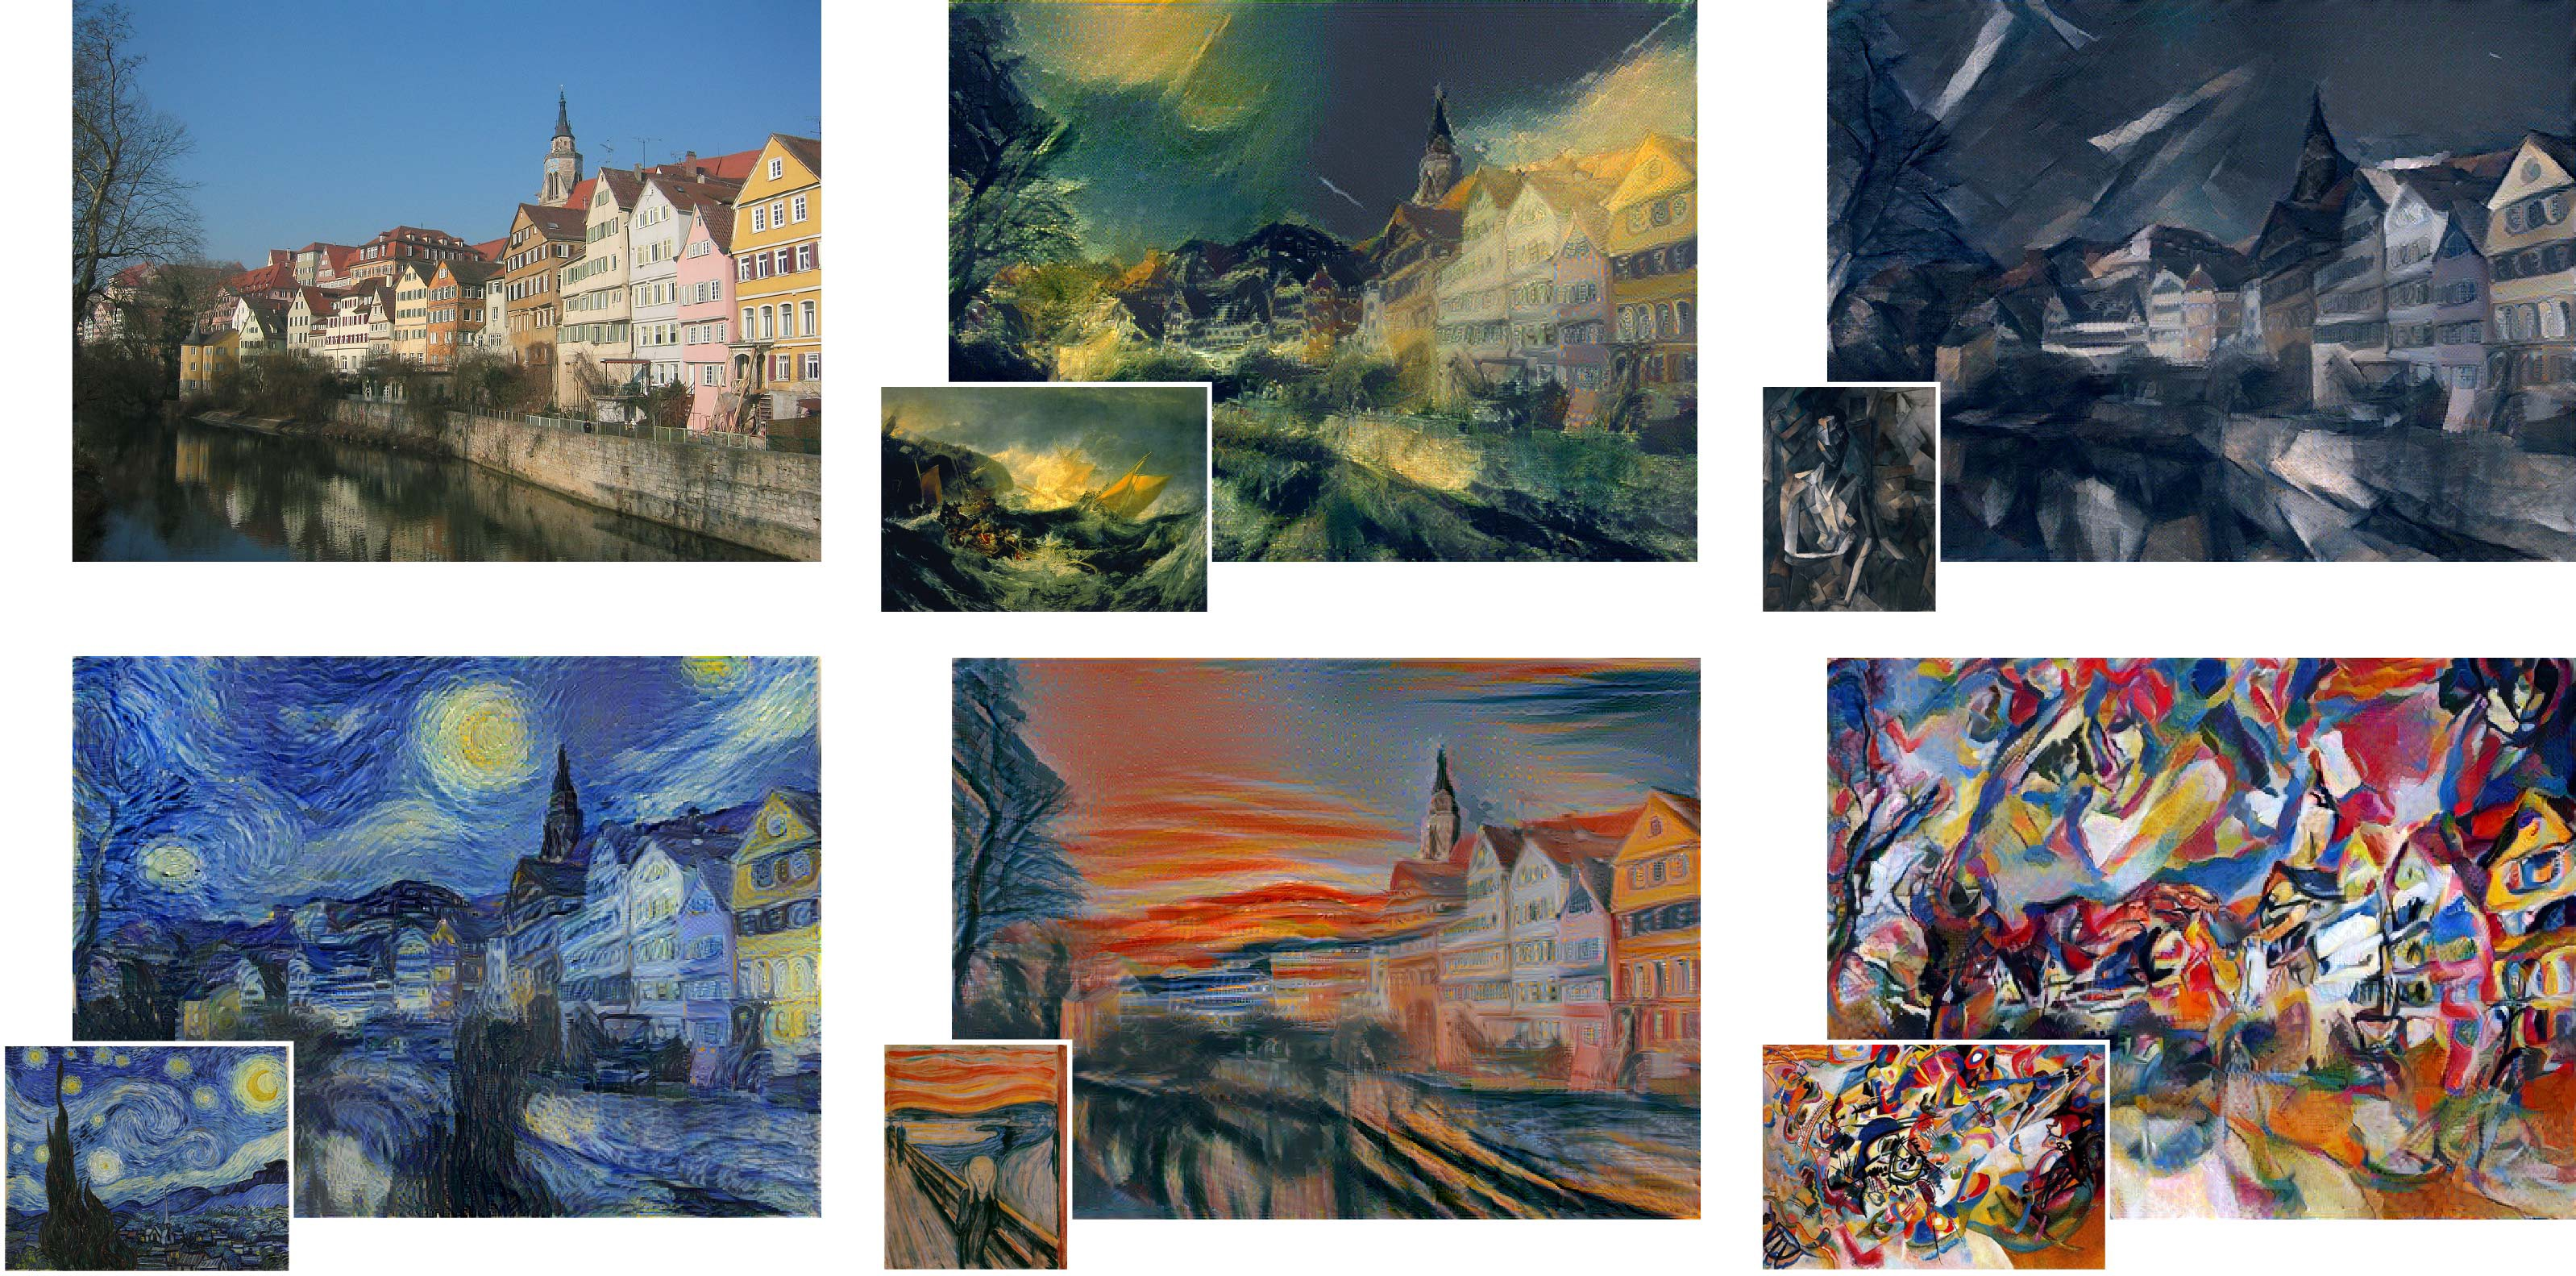
\includegraphics[width=6cm]{images/style-transfer.jpeg}
        \caption{Style transfer utilizando CycleGan
        \footnote{https://towardsdatascience.com/style-transfer-with-gans-on-hd-images-88e8efcf3716}.}
    \end{figure}


\end{frame}

\begin{frame}[fragile]{Introdução}

	A ideia geral por trás das GANs é utilizar duas redes neurais
	competindo uma com a outra, sendo uma rede responsável por
	gerar amostras parecidas com os dados reais (\textit{gerador})
	, enquanto a outra
	busca identificar quando o dado é real ou sintético
	(\textit{descriminador}).

    \begin{figure}[H]
        \centering
        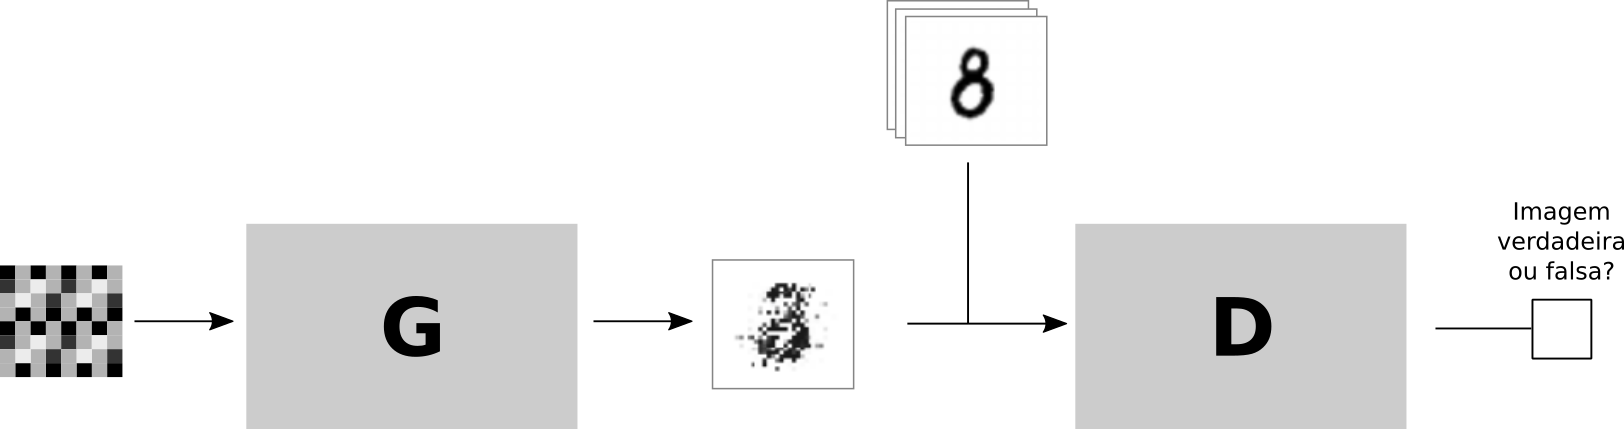
\includegraphics[width=10cm]{images/gan_scheme.png}
        \caption{Desenho esquemático de uma GAN "convencional".}
    \end{figure}

\end{frame}

\AtBeginSection{}
\section[Teoria]{Formalização Teórica}
\begin{frame}[fragile]{Formalização Teórica}
	Na formalização teórica da modelagem das 
	redes adversariais, consideraremos que
	o gerador e o descriminador são ambos \textit{multilayer perceptrons}.
	Os dados reais possuem uma distrbuição
	$p_{data}(\bm x)$, enquanto $p_g$ é a distribuição do gerador e
	$p_z(\bm z)$ é a priori do ruído de entrada. A função
	$G(\bm z, \theta_g)$ é a função diferenciável que transforma $\bm z$ no
	dado sintético, onde $\theta_g$ são os parâmetros da rede.
	A função $D(\bm x, \theta_d)$ retorna a probabilidade de $\bm x$ ter
	sido amostrada de $p_{data}$ invés de $p_g$.
	\begin{itemize}
		\item $p_g$ - Distribuição dos dados sintéticos;
		\item $p_z$ - Distribuição priori dos rúidos de entrada;
		\item $p_{data}$ - Distribuição real dos dados;
		\item $G(\bm z,\theta_g)$ - Função geradora;
		\item $D(\bm x,\theta_d)$ - Função discriminadora.
	\end{itemize}
\end{frame}


\begin{frame}[fragile]{Formalização Teórica}
	
	Nós treinamos $D$ buscando maximizar
	a capacidade de discernir dados de $p_{data}$ de $p_g$. Ao
	mesmo tempo que treinamos $G$ para minimizar $log(1-D(G(\bm z)))$.
	O treino da rede se resume ao problema de otimização dado
	pela seguinte função objetivo:
	\small
    $$
    \min_{G} \max_D V(D,G) =
    \mathbb{E}_{x\sim p_{data}(\bm x)}\left[\log{(D(\bm x))}\right]+
    \mathbb{E}_{z\sim p_z(\bm z)}\left[\log(1-D(G(\bm z))\right]
    $$

    \begin{figure}[H]
        \centering
        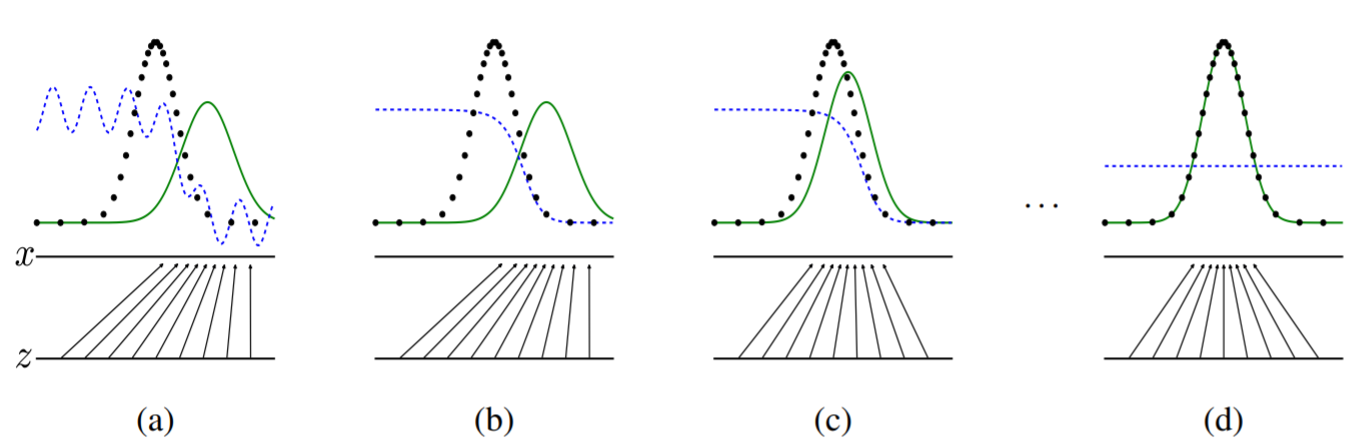
\includegraphics[width=8cm]{images/gan-algorithmscheme.png}
        \caption{De (a) até (d), o desenho ilustra a evolução do
        algoritmo ao ser treinado. A linha azul representa a
        distrbuição do descriminador, a linha verde representa
        a $p_g$, e os pontos pretos representam $p_{data}$
        \footnote{Imagem de \citet{goodfellow2014}}.}
    \end{figure}
	 
\end{frame}

\begin{frame}[fragile]{Formalização Teórica}

  \footnotesize
  \begin{algorithm}[H]
  \SetAlgoLined
  \For{número de iterações de treino}{
  	\For{k passos}{
  		Amostre $m$ valores $\{\bm z^{(1)},...,\bm z^{(m)} \}$
  		da priori $p_z(\bm z)$;

  		Amostre $m$ exemplos $\{\bm x^{(1)},...,\bm x^{(m)} \}$
  		da fução dos dados $p_{data}(\bm x)$;

  		Atualize o \textit{discriminator} utilizando
  		\textit{stochastic gradient descent}:
  		$$
  		\nabla_{\theta_d}\frac{1}{m}\sum^{m}_{i=1}
  		\left[
  		log D(\bm x^{(i)}) + log(1-D(G(\bm z^{(i)})))
  		\right]
  		$$
  	}

	Amostre $m$ valores $\{\bm z^{(1)},...,\bm z^{(m)} \}$
	da priori $p_z(\bm z)$;

	Atualize o \textit{generator} utilizando
	\textit{stochastic gradient descent}:
  		$$
  		\nabla_{\theta_d}\frac{1}{m}\sum^{m}_{i=1}
  		log(1-D(G(\bm z^{(i)})))
  		$$
  }
   \caption{GAN descrita em \citet{goodfellow2014}}
  \end{algorithm}

\end{frame}

\begin{frame}[fragile]{Formalização Teórica}
	
	Vamos estabelecer alguns resultados teóricos do funcionamento
	do algoritmo.

	\small
	\textbf{Proposição 1.} Para G fixo, o discriminador D ótimo é
	$
	D^*_G(\bm x) = \frac{p_{data}(\bm x)}
	{p_{data}(\bm x) + p_g(\bm x)}
	$.

	\hfill
	\break
	\textbf{Teorema 1.} O mínimo global da função objetivo
	é atingido se, e somente se, $p_g = p_{data}$. Neste ponto,
	o mínimo é $-log 4$.

	\hfill
	\break
	\textbf{Proposição 2.} Se G e D tiverem capacidade suficiente,
	e, em cada passo do Algortimo 1, o discriminador atingir o seu
	ótimo dado G com $p_g$ sendo atualizado para melhorar o critério
    $$
    \mathbb{E}_{x\sim p_{data}(\bm x)}\left[\log{(D(\bm x))}\right]+
    \mathbb{E}_{z\sim p_z(\bm z)}\left[\log(1-D(G(\bm z))\right]
    $$
    então $p_g$ converge para $p_{data}$.

\end{frame}

\begin{frame}[fragile]{Formalização Teórica}
\small
	\textbf{Proposição 1.} Para G fixo, o discriminador D ótimo é
	$
	D^*_G(\bm x) = \frac{p_{data}(\bm x)}
	{p_{data}(\bm x) + p_g(\bm x)}
	$.

	\textit{Demonstração:}
	\hrule
  $$V(D,G)=
    \mathbb{E}_{x\sim p_{data}(\bm x)}\left[\log{(D(\bm x))}\right]+
    \mathbb{E}_{z\sim p_z(\bm z)}\left[\log(1-D(G(\bm z))\right]
  $$
  \pause
  $$= \int_x p_{data}(x)\log{(D(x))}dx + \int_z p_z(z)\log{(1-D(G(z)))}dz $$
  \pause
  $$x = G(z) \implies z = G^{-1}(x) \implies dz = (G^{-1})'(x)dx $$
  $$p_g(x) = p_z(G^{-1}(x))(G^{-1})'(x)dx $$
  \pause
  $$= \int_x p_{data}(x)\log{(D(x))}dx + \int_x p_z(G^{-1}(x))\log{(1-D(x))}(G^{-1})'(x)dx $$
  \pause
  $$= \int_x p_{data}(x)\log{(D(x))}dx + \int_x p_g(x)\log{(1-D(x))}dx $$
  \pause
  $$= \int_x p_{data}(x)\log{(D(x))} + p_g(x)\log{(1-D(x))}dx $$
\end{frame}

\begin{frame}[fragile]{Formalização Teórica}
\small
	\textbf{Proposição 1.} Para G fixo, o discriminador D ótimo é
	$
	D^*_G(\bm x) = \frac{p_{data}(\bm x)}
	{p_{data}(\bm x) + p_g(\bm x)}
	$.

	\textit{Demonstração:}
	\hrule
 $$\max_{D} V(D,G) = \max_{D}\int_x p_{data}(x)\log{(D(x))} + p_g(x)\log{(1-D(x))}dx $$
 \pause
 $$\frac{\partial}{\partial D(x)} \left(p_{data}(x)\log{(D(x))} + p_g(x)\log{(1-D(x))}\right) = 0 $$
 \pause
 $$\implies \dfrac{p_{data}(x)}{D(x)} - \dfrac{p_g(x)}{1 - D(x)} = 0 $$
 $$\implies D(x) = \dfrac{p_{data}(x)}{p_{data}(x)+p_g(x)} $$
 \QEDB
\end{frame}

\begin{frame}[fragile]{Formalização Teórica}

	\textbf{Teorema 1.} O mínimo global da função objetivo
	é atingido se, e somente se, $p_g = p_{data}$. Neste ponto,
	o mínimo é $-log4$.

	\textit{Demonstração:}
	\hrule

	$
	\implies )$
	Seja $p_g = p_{data}, D^*_G(x) = \frac{1}{2}$. Assim,

  $$V(D,G)=
    \mathbb{E}_{x\sim p_{data}(\bm x)}\left[log (1/2) \right]+
    \mathbb{E}_{x\sim p_g(\bm x)}\left[log(1/2)\right] =  -log4
  $$


\end{frame}

\begin{frame}[fragile]{Formalização Teórica}

\small
	\textbf{Teorema 1.} O mínimo global da função objetivo
	é atingido se, e somente se, $p_g = p_{data}$. Neste ponto,
	o mínimo é $-log4$.

	\textit{Demonstração:}
	\hrule

	$
	\impliedby )$ Seja $C(G) = \max_{D}V(G,D)$, assim
  $$C(G) = \int_{x}p_{data}(x)\log{\left(D_{G}^{*}(x)\right)}
  + p_{g}(x)\log{\left(1-D_{g}^{*}(x)\right)}dx $$
  \pause
  $$
  = \int_{x}p_{data}(x)\log{\left(\dfrac{p_{data}(x)}{p_{data}(x)
  + p_{g}(x)}\right)} + p_{g}(x)\log{\left(\dfrac{p_{g}(x)}{p_{data}(x)
  + p_{g}(x)}\right)}dx $$
  \pause
  $$= \int_{x}p_{data}(x)
  \log{\left(2^{-1}\cdot \dfrac{p_{data}(x)}{\dfrac{p_{data}(x)
  + p_{g}(x)}{2}}\right)} + p_{g}(x)
  \log{\left(2^{-1}\cdot \dfrac{p_{g}(x)}{\dfrac{p_{data}(x)
  + p_{g}(x)}{2}}\right)}dx	$$
  \pause
  $$=
    \mathbb{E}_{x\sim p_{data}(\bm x)}\left[-\log (2)+
    \frac{p_{data}(x)}{p_{data}(x)+p_g(x)}\right]+
    \mathbb{E}_{x\sim p_g(\bm x)}\left[-\log(2)+
    \frac{p_{g}(x)}{p_{data}(x)+p_g(x)}\right]
  $$

\end{frame}

\begin{frame}[fragile]{Formalização Teórica}

\small
	\textbf{Teorema 1.} O mínimo global da função objetivo
	é atingido se, e somente se, $p_g = p_{data}$. Neste ponto,
	o mínimo é $-log4$.

	\textit{Demonstração:}
	\hrule
  $$C(G) = KL\left[p_{data}(x)||\dfrac{p_{data}(x)+p_g(x)}{2}\right] + KL\left[p_g(x)||\dfrac{p_{data}(x) + p_g(x)}{2}\right] - \log{4} $$
  $$= 2 \cdot JSD\left[ p_{data} \mid \mid p_g
  \right] - \log 4$$

  Onde $KL$ é a distância Kullback-Leibler e $JSD$ é a divergência
  de Jensen-Shannon. Assim:
  $$\min_G C(G) = \min_G \left( 2 \cdot JSD\left[ p_{data} \mid \mid p_g
  \right] - \log 4 \right)$$
  O mínimo da divergência $JSD$ é zero e só é atingido se, e somente se,
  $p_g = p_{data}$\footnote{Estamos assumindo que o modelo
  generativo é capaz de reproduzir perfeitamente a distribuição dos
  dados}. \QEDB
\end{frame}

\begin{frame}[fragile]{Formalização Teórica}
	
	\small
	\textbf{Proposição 2.} Se G e D tiverem capacidade suficiente,
	e, em cada passo do Algortimo 1, o discriminador atingir o seu
	ótimo dado G com $p_g$ sendo atualizado para melhorar o critério
    $$
    \mathbb{E}_{x\sim p_{data}(\bm x)}\left[\log{(D(\bm x))}\right]+
    \mathbb{E}_{x\sim p_g(\bm x)}\left[1-\log{(D(\bm x))}\right]
    $$
    então $p_g$ converge para $p_{data}$.

	\textit{Demonstração:}
	\hrule

	Considere $V(G,D) = U(p_g,D)$. Assim, para um $D$ fixo, $U$ é
	função de $p_g$. Note que $U(p_g,D)$ é convexo, pois
	$$ U(p_g,D) = 
    \mathbb{E}_{x\sim p_{data}(x)}\left[\log{(D(x))}\right]+
    \mathbb{E}_{x\sim p_g(x)}\left[1-\log{(D(x))}\right] \therefore
	$$
	\pause
	$$U(\alpha p + (1-\alpha)q,D) = 
	\int_x \alpha\cdot p(x)\log{(D(x))} + (1-\alpha)q(x)\log{(1-D(x))}dx
	$$
	$$
	=
    \alpha\mathbb{E}_{x\sim p(x)}\left[\log{(D(x))}\right]+
    (1-\alpha)\mathbb{E}_{x\sim q(x)}\left[1-\log{(D(x))}\right]
	$$
	$$
	= \alpha U(p,D) + (1-\alpha)U(q,D)
	$$

\end{frame}

\begin{frame}[fragile]{Formalização Teórica}
	
	\small
	\textbf{Proposição 2.} Se G e D tiverem capacidade suficiente,
	e, em cada passo do Algortimo 1, o discriminador atingir o seu
	ótimo dado G com $p_g$ sendo atualizado para melhorar o critério
    $$
    \mathbb{E}_{x\sim p_{data}(\bm x)}\left[\log{(D(\bm x))}\right]+
    \mathbb{E}_{x\sim p_g(\bm x)}\left[1-\log{(D(\bm x))}\right]
    $$
    então $p_g$ converge para $p_{data}$.

	\textit{Demonstração:}
	\hrule

	Como $U(p_g,D)$ é um função convexa, podemos utilizar um algoritmo
	de descida de gradiente para atingir o seu mínimo no ponto
	onde esse gradiente é igual a zero, e que como provado
	no \textbf{Teorema 1}, é um mínimo global.
	\QEDB
	\pause

	\textcolor{red}{Na prática, a GAN otimiza os parâmetros
	$\theta_g$ invés de $p_g$, então a prova não se aplica,
	já que o \textit{mulilayer perceptron} aproxima um subconjunto
	da família de $p_g$.}

\end{frame}

\AtBeginSection{}
\section[Variações]{Variações}
\begin{frame}[fragile]{Variações}

	Além do modelo tradicional apresentado, variações de GANs
	tem surgido para diferentes aplicações.

	\begin{itemize}
		\item \textbf{DCGAN}: Uso de Convolutional Neural Networks
		em GANs para melhorar o processo de geração de dados sintéticos.
		\item \textbf{Face Inpainting}: Utilização de GANs para
		"reconstrução" de imagens com partes faltantes.

    \begin{figure}[H]
        \centering
        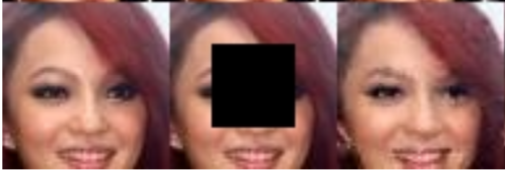
\includegraphics[width=4cm]{images/gan-inpainting.png}
        \caption{Inpainting usando GAN \citep{yeh2017}.}
    \end{figure}

		\item \textbf{Transferência Imagem-Imgeam}:
		Utilização de GANs para transformar um grupo de imagens
		em outro, como no exemplo de transferência de estilo.


	\end{itemize}

\end{frame}

\begin{frame}[fragile]{Variações}

	A arquitetura \textbf{CycleGAN} \citep{zhu2017} é uma das
	mais utilizadas para transferências imagem-imagem.
    \begin{figure}[H]
        \centering
        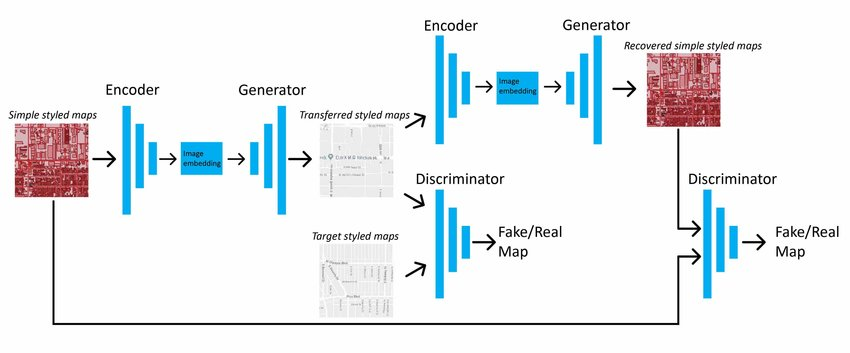
\includegraphics[width=10cm]{images/gan-cyclearch.jpg}
        \caption{Architetura de uma CycleGAN \citep{kang2019}.}
    \end{figure}

\end{frame}

\AtBeginSection{}
\section[Problemas Típicos]{Problemas Típicos}
\begin{frame}[fragile]{Problemas Típicos}
GANs tradicionais possuem falhas comuns que tem sido foco
de pesquisas. \citet{arjovsky2017} clarificaram a fonte desses
problemas e propuseram algumas soluções.
\small
\begin{itemize}
	\item \textbf{Dissipação de gradientes:} Na prática, ao treinar
	o descriminador até seu estado ótimo ($\frac{p_{data}}
	{p_{data} + p_g}$), os gradientes tendem a se dissipar
	no treinamento do gerador
  $$\lim_{||D-D^*||\to0}\nabla_{\theta}\mathbb{E}_{z~p(z)}\left[\log{(1-D(G_{\theta}(z)))}\right] = 0$$

  \item  \textbf{``Mode Colapse"}: Normalmente, você deseja que sua GAN
  produza uma ampla variedade de saídas. No entanto, se um gerador produz
  uma saída especialmente plausível, ele pode aprender a produzir apenas
  essa saída.

  \item \textbf{Falha de Converêgncia}: GANs podem apresentar instabilidade
  na atualização dos gradientes do gerador, levando a falhas de
  convergência.
\end{itemize}

\end{frame}

\begin{frame}[fragile]{Problemas Típicos}
Soluções propostas para esses problemas são:
\small
\begin{itemize}
	\item \textbf{Dissipação de gradientes:}
	\begin{enumerate}
		\item Alterar a função objetivo do gerador para
		$C(G) = \max \log(D^*(G(z)))$ \citep{goodfellow2014}.
		\item WGAN - Utilizar métrica Wasserstein, definida abaixo,
		como função objetivo \citep{wgan2017}.
	\end{enumerate}

  \item  \textbf{``Mode Colapse"}:
	\begin{enumerate}
		\item WGAN.
	\end{enumerate}

  \item \textbf{Falha de Converêgncia}:
	\begin{enumerate}
		\item Adicionar ruído nas entradas do discriminador.
  
  		\item Penalizar pesos do Discriminador.

	\end{enumerate}
\end{itemize}

\end{frame}


\begin{frame}[allowframebreaks]{References}

% \renewcommand{\bibsection}{\section{}}
  \renewcommand{\section}[2]{}%
  \bibliography{gan}
  % \bibliographystyle{plainnat}
  % \bibliographystyle{plain}
  % \bibliographystyle{abbrv}
  \bibliographystyle{apa}

\end{frame}

\AtBeginSection{}
\section[Anexo]{Anexo}
\begin{frame}[fragile]{Anexo}
	Neste anexo apresentamos mais informações sobre o problema de 
	dissipação de gradientes e a solução utilizandos WGAN.

  \small
  \textbf{Solução para Dissipação de Gradientes:}\\
  (i) Alterar a função objetivo do gerador para $C(G) = \max -\log(D^*(G(z)))$. Dessa, forma foi provado que
  $$\mathbb{E}_{z~p(z)}\left[-\nabla_{\theta}\log{D^*(G_{\theta}(z))|_{\theta=\theta_{0}}} \right] = \nabla_{\theta}[KL(p_{g_{\theta}}||p_{data}) - 2JSD(p_{g_{\theta}}||p_{data})]|_{\theta = \theta_0} $$
  Note que: \\
  a. JSD's estão com sinais opostos. Significa que estão pressionando para que as distribuições sejam diferentes, o que parece ser uma falha na atualização.\\
  b. $KL(p_{g_{\theta}}||p_{data})$ não é equivalente ao da máxima verossimilhança.\\
  Isso explica porque os GANs (quando estabilizados) criam amostras de boa aparência e justifica porque os GANs sofrem com uma quantidade grande de "Mode Dropping".
\end{frame}

\begin{frame}[fragile]{Anexo}
  \small
  \textbf{Solução para Dissipação de Gradientes:}\\
  (ii) (WGAN) - Utilizar métrica Wasserstein, definida abaixo, como função objetivo.
  $$W(p_{data},p_g) = \inf_{\gamma\in\Gamma(p_{data},p_g)}\mathbb{E}_{(x,y)~\gamma}[||x-y||] $$
  \pause
  Porém, implementar essa definição é impraticável. Em seu lugar, através da dualidade Kartrovich - Rubinstein, podemos aproximá-la por
  $$W(p_{data},p_g) = \sup_{||f||_L\leq1} \frac{1}{K}\mathbb{E}_{x~p_{data}}[f(x)]- \mathbb{E}_{x~p_g}[f(x))]$$
  \pause
  Suponha que $f$ pertença à família de funções K-Lipschitz $\{f_w\}_{w \in W}$. Temos então
  $$W(p_{data},p_g) = \max_{w \in W} \mathbb{E}_{x~p_{data}}[f_w(x)] - \mathbb{E}_{z~p_z}[f_w(G(z))] \text{, tal que } ||f_w||_L \leq K$$
  \pause
  O Discriminador é usado para aprender $w$ e encontrar $f_w$. A função $W$ então se torna.
  $$W(p_{data},p_g) = \max_{w \in W} \mathbb{E}_{x~p_{data}}[D_w(x)] - \mathbb{E}_{z~p_z~}[D_w(G(z))] \text{, tal que } ||D_w||_L \leq K$$
\end{frame}

\begin{frame}[fragile]{Anexo}
  \small
  Dessa forma, D deixa de ser um Discriminador (com saída [0,1]) que buscava descobrir quais amostras são falsas ou verdadeiras e se transforma em um Crítico (com saída $\geq0$), treinado para aprender funções contínuas K-Lipschitz que ajudarão a computar a métrica Wasserstein. \\
  A função objetivo da nova GAN (WGAN) passa a ser então.
  $$V(G,D) = \min_{\theta} \max_{w \in W} \mathbb{E}_{x~p_{data}}[D_w(x)] - \mathbb{E}_{z~p_z~}[D_w(G_{\theta}(z))] \text{, tal que } ||D_w||_L \leq K$$
  Uma vez que a métrica Wasserstein tem um comportamento suave ela elimina o problema da dissipação do gradiente.
\end{frame}


\end{document}
